\documentclass[tikz,border=10pt]{standalone}
% no extra packages needed beyond TikZ defaults
\begin{document}
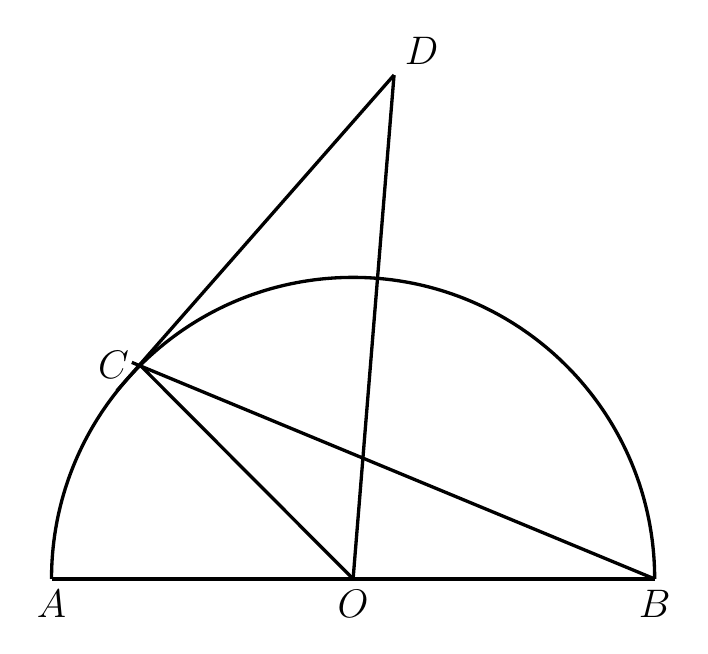
\begin{tikzpicture}[line width=1.2pt, line join=round,
    every node/.style={font=\fontsize{13.5}{16.2}\selectfont}]
  % Named coordinates (scale s = 0.010855 cm per px, y flipped, O at origin)
  \coordinate (O) at (0,0);
  \coordinate (A) at (-3.83,0);
  \coordinate (B) at (3.83,0);
  \coordinate (C) at (-2.71,2.72);
  \coordinate (D) at (0.52,6.40);
  \coordinate (P1) at (-2.81,2.75);  % line B-C extended
  \coordinate (P2) at (-3.00,2.39);  % line D-C extended

  % Upper semicircle from A over the top to B (clockwise from 180 deg to 0 deg)
  \draw (A) arc[start angle=180, delta angle=-180, radius=3.83];

  % Diameter AB
  \draw (A) -- (B);

  % Segments from O
  \draw (O) -- (D);
  \draw (O) -- (C);

  % Line through B and C, extended to P1
  \draw (B) -- (P1);

  % Line through D and C, extended to P2
  \draw (D) -- (P2);

  % Labels in serif (default font), offset away from the figure
  \node[below] at (A) {$A$};
  \node[below] at (B) {$B$};
  \node[below] at (O) {$O$};
  % D label moved above the vertex (above right), as in the original
  \node[above right] at (D) {$D$};
  \node[left]  at (C) {$C$};
\end{tikzpicture}
\end{document}